\section{Validation}

\begin{frame}\frametitle{\secname}
\underline{Recall}:
    \notesonly{
    Among the requirements for fitting a model to a desired function $y(\vec x; \vec w)$ was having a
    }
    performance measure, a criterion for \emph{model selection}.
    \mode<article>{Specifically, \\

    the generalization \textbf{error} $E^G$ which is defined as:}	
    \begin{equation} 
                \EGw \; := \; \left<\,e\,\right>_{y_T, \vec{x}; \vec w} 
                \; = \; \iint d \vec{x} \, dy_T \; 
                    P{(y_T, \vec{x})} \, e{\tyxw}
    \end{equation}
    \pause
    Because $P{(y_T, \vec{x})}$ is not known, \mode<article>{applying empirical risk minimization (ERM)
    enables us to approximate $\EGw$ by computing the} empirical average $\ETw$ using the available training data:
    $$
    \left\{\left(\vec x^{(\alpha)}, y_T^{(\alpha)}\right)\right\}, \alpha=1,\ldots,p.
    $$
    \mode<article>{The training error $\ETw$ becomes:}

    \mode<presentation>{\vspace{-5mm}}
    \begin{equation}
    \text{batch training error:}\quad \ETw=\frac{1}{p}\sum_{\alpha=1}^{p} \underbrace{e\tyxwalpha}_{e^{(\alpha)}}
    \end{equation}
    \mode<presentation>{
    or mini-batch and stochastic online approximations of $E^T_{[\vec w]}$ 
    }
    \mode<article>{
    where $e\tyxwalpha$ (or $e^{(\alpha)}$ for brevity) is the cost computed from the prediction for a specific observation $y(\vec x^{(\alpha)};\vec w)$ and its corresponding label $y_T^{(\alpha)}$. The superscript $^{(\alpha)}$ is used to index a specific point (sample) in the dataset.
    We have also seen that $E^T$ can be further approximated by changing its ``scope'' to a set of samples in a mini-batch or a single randomly selected sample (i.e. stochastic online learning)
    
    This leaves us with the question:
    }
    
    \question{How well does $E^T$ represent $E^G$?}
    
\end{frame}

\begin{frame}
\mode<article>{
We will now focus on:
}
\mode<presentation>{
Today:
}
\begin{enumerate}
\item Diagnostics for how well $E^T$ represents $E^G$
\item Improving estimates for the generalization error $E^G$
\item Common methods for improving generalization error $E^G$, doing better on unseen data (e.g. regularization)
\end{enumerate} 

\end{frame}


\begin{frame}

\notesonly{
Optimizing model parameters to training data and obtaining some solution }$\vec w^* = \argmin_{\vec w} E^T_{[\vec w]}$ does not imply good generalization performance.

\begin{equation}
\text{small} \;\; E^T_{[\vec w^*]} \quad \cancel{\Rightarrow}\quad \text{small} \;\;  E^G_{[\vec w^*]}
\end{equation}
Expected:
\begin{equation}
E^T_{[\vec w^*]} \quad <\quad E^G_{[\vec w^*]}
\end{equation}

Validation: evaluate the generalization of a model (and its training procedure) by estimating

\begin{equation}
\widehat E^G_{[\vec w]} \approx E^G_{[\vec w]} = \iint d \vec x \, d  y P(\vec x,  y_T) \, e( y(\vec x; \vec w), y_T) 
\end{equation}

\notesonly{The above is }not limited to scalar attributes $y$, $y_T$\notesonly{ and extends to $\vec y$, $\vec y_T \in \R^M$}.\\

\pause
This implies that we need a set of data.
\pause
\notesonly{It is very important that we do not use this data for training the model. This data has to be completely excluded from the model selection process.

We use the original training set $\{\vec x_{\text{train}}^{(\alpha)}, {y_T}_{\text{train}}^{(\alpha)}\}_{\alpha=1}^{p}$ for model selection.
Model selection uses the training data to find $\vec w^* = \argmin_{\vec w} E^T_{[\vec w]}$. 

We use the new hold-out set to \emph{validate} ($\{\vec x_{\text{val.}}^{(\beta)}, {y_T}_{\text{val.}}^{(\beta)}\}_{\beta=1}^{q}$) to estimate the generalization error for this particular solution (i.e. $\widehat E^G_{[\vec w^*]})$
}
\slidesonly{
\begin{itemize}
\item $\{\vec x_{\text{train}}^{(\alpha)}, {y_T}_{\text{train}}^{(\alpha)}\}_{\alpha=1}^{p}$ for model selection
\item $\leadsto \vec w^* = \argmin_{\vec w} E^T_{[\vec w]}$
\pause
\item $\{\vec x_{\text{val.}}^{(\beta)}, {y_T}_{\text{val.}}^{(\beta)}\}_{\beta=1}^{q}$ for validation
\pause
\item $\widehat E^G_{[\vec w^*]}$
\end{itemize}
}


\end{frame}

\mode<article>{
Let us look at the following scenario where we've trained 
}

\subsection{Overfitting vs. Underfitting}

% -----------------------------------------------------------------------------
\begin{frame}\frametitle{\subsecname}
	\begin{tabular}{c c}
		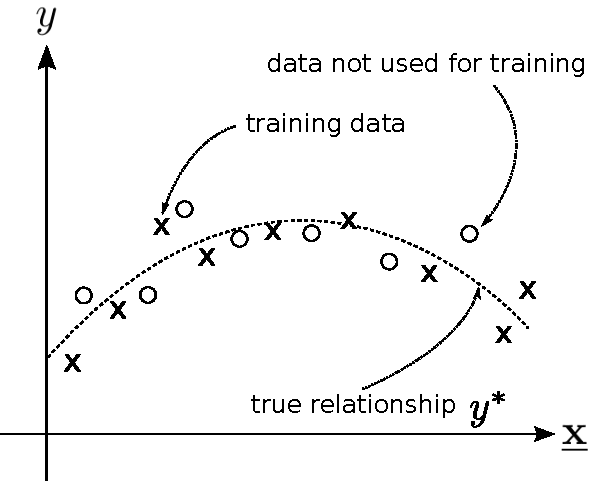
\includegraphics[height=5cm]{img/section1_fig27} & 
		\raisebox{2.5cm}{
			\begin{tabular}{l}
				data generation: \\
				e.g.~$y_T \;=\;\; y_{(\vec{x};\vec w)}^* \;\;
				+ \kern-2ex\underbrace{\eta}_{\begin{array}{c}
					\text{\scriptsize noise,}\\[-2mm] 
					\text{\scriptsize zero mean} 
				\end{array}}$
			\end{tabular}
		}
	\end{tabular}
\end{frame}

% -----------------------------------------------------------------------------
\definecolor{darkgreen}{rgb}{0,0.6,0}
\begin{frame} \frametitle{\subsecname}
Compare ${\color{red}E^T}$ and ${\color{darkgreen} \widehat E^G}$:\\

	\begin{minipage}{3.5cm}
	\begin{center}
		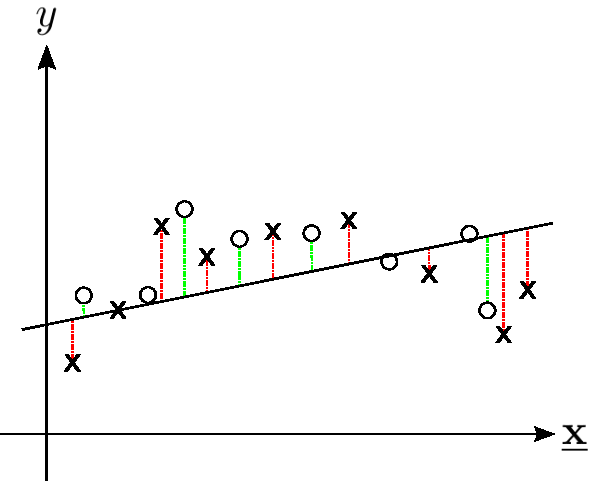
\includegraphics[height=4cm]{img/section1_fig28}
	\end{center}
	\pause
	\begin{equation}
			\left.
			\begin{array}{l}
			  {\color{red}E^T} \text{ large} \\
			  {\color{darkgreen} \widehat E^G} \text{ large}
			\end{array} \right \} {\color{red}E^T} \approx {\color{darkgreen} \widehat E^G}
	\end{equation}
	\end{minipage}
	\pause
	\hspace{2.5cm}
	\begin{minipage}{3.5cm}
	\begin{center}
		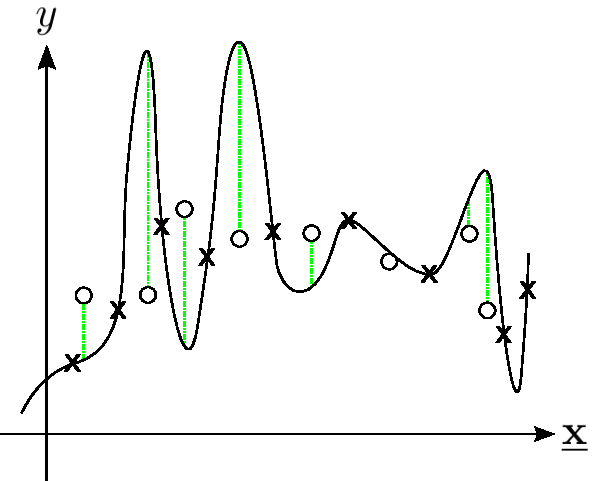
\includegraphics[height=4cm]{img/section1_fig30}
	\end{center}
	\pause
	\begin{equation}
			\left. \begin{array}{l}
				{\color{red}E^T} \text{ small} \\
				{\color{darkgreen} \widehat E^G} \text{ large}
			\end{array} \right \} {\color{red}E^T} \ll {\color{darkgreen}\widehat E^G}
	\end{equation}
	\end{minipage}
\end{frame}


% -----------------------------------------------------------------------------
\begin{frame}\frametitle{Well fitted model} 
	\begin{center}
		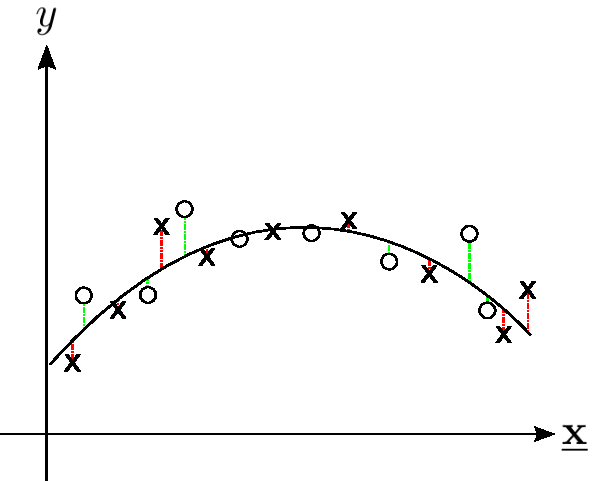
\includegraphics[height=4cm]{img/section1_fig29}
	\end{center}

	\begin{block}{Diagnostics}
		$$
			\left. \begin{array}{l}
				{\color{red}E^T} \text{ small} \\
				 {\color{darkgreen}\widehat E^G} \text{ small}
			\end{array} \right \} {\color{red}E^T} \approx {\color{darkgreen}\widehat E^G}
		$$
	\end{block}
\end{frame}


% -----------------------------------------------------------------------------
\begin{frame}\frametitle{Underfitting} 
\slidesonly{
	\begin{minipage}{2cm}
	\begin{center}
		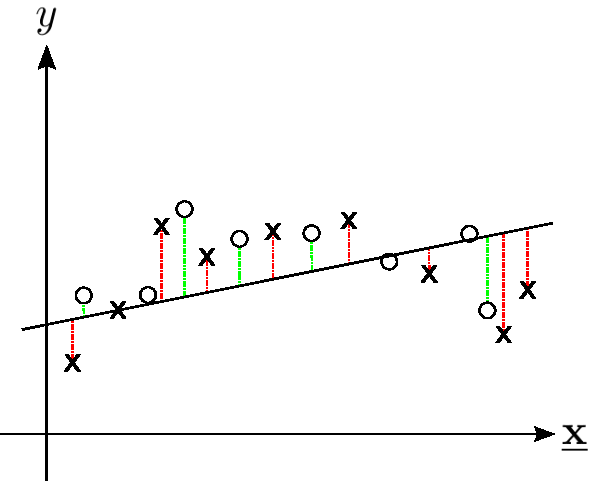
\includegraphics[height=3cm]{img/section1_fig28}
	\end{center}
	\begin{equation}
			\left.
			\begin{array}{l}
			  {\color{red}E^T} \text{ large} \\
			  {\color{darkgreen} \widehat E^G} \text{ large}
			\end{array} \right \} {\color{red}E^T} \approx {\color{darkgreen} \widehat E^G}
	\end{equation}
	\end{minipage}
	\hspace{2.5cm}
}
	\pause
%\slidesonly{
	\begin{minipage}{\slidesonly{6cm}\notesonly{11cm}}
	
\question{What is underfitting?}

	\begin{itemize}
	\item function complexity \notesonly{>}\slidesonly{vs.} model complexity \notesonly{(e.g. fitting a parabola using only a straight line, fitting a sinusoid using a parabola)}
	\item the degrees of freedom in the model are too ...\notesonly{low}
	
	\pause
	
	\item the model is insensitive to variations in the features
	\end{itemize}

	\end{minipage}

\question{How would replacing a few training samples change the solution?} 
	
	\pause
	
	- Not much.

\end{frame}

\begin{frame}\frametitle{Overfitting} 
\slidesonly{
	\begin{minipage}{2cm}
	\begin{center}
		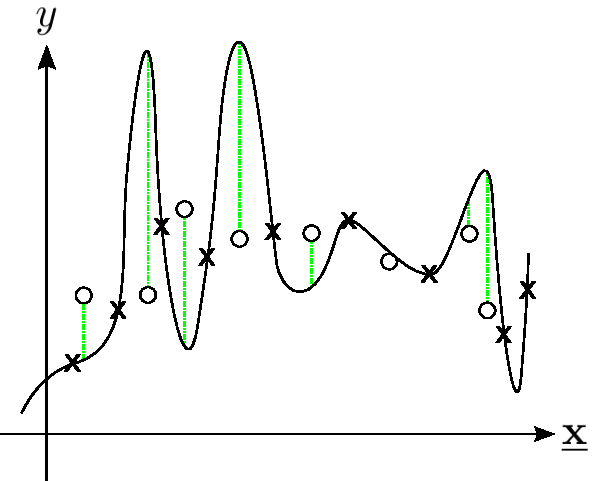
\includegraphics[height=3cm]{img/section1_fig30}
	\end{center}
	\begin{equation}
			\left. \begin{array}{l}
				{\color{red}E^T} \text{ small} \\
				{\color{darkgreen} \widehat E^G} \text{ large}
			\end{array} \right \} {\color{red}E^T} \ll {\color{darkgreen}\widehat E^G}
	\end{equation}
	\end{minipage}
	\hspace{2cm}
}
	\pause
%\slidesonly{
	\begin{minipage}{\slidesonly{6cm}\notesonly{11cm}}
	
\question{What is overfitting?}

	\begin{itemize}
	\item function complexity \notesonly{<}\slidesonly{vs.} model complexity \notesonly{(e.g. fitting a line using a parameterized sinusoid, using an MLP with non-linear functions to fit a straight line.}
	
	\pause
	
	\item the degrees of freedom in the model are...\notesonly{unnecessarily high}
	
	\pause
	
	\item the model is over-sensitive to the noise component
	\item the model has ``memorized'' the training data instead of learning a representation for it.
	\end{itemize}
	

	\end{minipage}


	\question{How would replacing a few training samples change the solution?} 
	
	\pause
	- A lot.

\end{frame}

\subsubsection{Dealing with overfitting/underfitting}

\mode<presentation>{
\begin{frame}{\subsubsecname}

\slidesonly{\vspace{-2mm}}
\begin{table}[h]
\begin{tabular}{r|r|c|c|}
\hline
&          reduces $\rightarrow$                                                       & \begin{tabular}[c]{@{}c@{}} overfitting\end{tabular} & \begin{tabular}[c]{@{}c@{}}underfitting\end{tabular} \\ \hline
1&more training data                                                                        &                                                            &                                                              \\ \hline
2&\begin{tabular}[c]{@{}r@{}}larger reg.\\ coeff. $\lambda$\end{tabular}   &                                                            &                                                              \\ \hline
3&\begin{tabular}[c]{@{}r@{}}smaller reg.\\ coeff. $\lambda$\end{tabular}  &                                                             &                                                             \\ \hline
4&use a more complex model                                                             &                                                             &                                                             \\ \hline
5&use a simpler model                                                                  &                                                            &                                                              \\ \hline
6&\begin{tabular}[c]{@{}r@{}}increase no. of\\ hidden neurons in MLP\end{tabular} &                                                             &                                                             \\ \hline
7&\begin{tabular}[c]{@{}r@{}}add more hidden\\ layers to MLP\end{tabular}            &                                                             &                                                             \\ \hline
8&\begin{tabular}[c]{@{}r@{}}add features\\ to the input $\vec x$\end{tabular}            &                                                             &                                                             \\ \hline
9&\begin{tabular}[c]{@{}r@{}}shuffle the data\end{tabular}            &                                                             &                                                             \\ \hline
\end{tabular}
\end{table}

\end{frame}

}

\begin{frame}{\subsubsecname}
\slidesonly{\vspace{-2mm}}
\notesonly{Assuming one has performed diagnostics of comparing $E^T$ and $\widehat E^G$ to identify if a model is overfitting or underfitting. How would one mitigate one or the other?\\

}

\begin{center}
\begin{table}[h]
\begin{tabular}{r|r|c|c|}
\hline
&          \underline{\textbf{potentially}} reduces $\rightarrow$                                                       & \begin{tabular}[c]{@{}c@{}} overfitting\end{tabular} & \begin{tabular}[c]{@{}c@{}}underfitting\end{tabular} \\ \hline
1&more training data                                                                           & yes                                                           & no                                                             \\ \hline
2&\begin{tabular}[c]{@{}r@{}}larger regularization\\ coeff. $\lambda$\end{tabular}   & yes                                                           & no                                                             \\ \hline
3&\begin{tabular}[c]{@{}r@{}}smaller regularization\\ coeff. $\lambda$\end{tabular}  & no                                                            & yes                                                            \\ \hline
4&use more complex model                                                             & no                                                            & yes                                                            \\ \hline
5&use simpler model                                                                  & yes                                                           & no                                                             \\ \hline
6&\begin{tabular}[c]{@{}r@{}}increase number of\\ hidden neurons in MLP\end{tabular} & no                                                            & yes                                                            \\ \hline
7&\begin{tabular}[c]{@{}r@{}}add more hidden\\ layers to MLP\end{tabular}            & no                                                            & yes                                                            \\ \hline
8&\begin{tabular}[c]{@{}r@{}}add features\\ to the input $\vec x$\end{tabular}            & no                                                            & yes                                                            \\ \hline
9&\begin{tabular}[c]{@{}r@{}}shuffle the data\end{tabular}         &   no                                                            & no
                                                                 \\ \hline
&more techniques?                                                                   &                                                               &                                                                \\ \hline
\end{tabular}
\end{table}
\end{center}

\end{frame}

\subsubsection{Different views of the bias-variance tradeoff}

\begin{frame}{\subsubsecname}

\notesonly{
\textbf{Remember: it's always a bias-variance \underline{tradeoff}}\\

The above ``fixes'' rely on having concluded that the model is either overfitting or underfitting. And that this can potentially be mitigated by taking these different measures. However, it is important to understand how overfitting and underfitting reflect where we are on the bias-variance tradeoff. This means that repeatedly applying one solution to an overfitting model can eventually cause the model to underfit and vice-versa. One should also note that if one of the above doesn't work. It does not conclude that the model was not overfitting or underfitting. The above are simply guidelines on how to understand why a model has poor generalization performance and come up with simple techniques for finding a different bias-variance tradeoff.

Although we've just talked about how increasing the size of the training set can help mitigate overfitting. Observing how $E^T$ and $\widehat E^G$ behave as a function of the training set size $p$ is a way of determining if an overfitting problem even exists. Keep in mind that $\widehat E^G$ would not directly depend on the size of the training set as it is only evaluated on the hold-out set, which we won't change in size. Nevertheless, every time we train our model with a larger training set, we evaluate both $E^T$ and $\widehat E^G$ for this trained model.
}

Using a larger training set (i.e. increasing $p$) to identify potential overfitting vs. underfitting of the model:

\question{What $E^T$ vs. $p$ relationship do we expect for an \emph{underfitting} model?}

\question{What $E^T$ vs. $p$ relationship do we expect for an \emph{overfitting} model?}

\question{What $\widehat E^G$ vs. $p$ relationship do we expect for an \emph{underfitting} model?}

\question{What $\widehat E^G$ vs. $p$ relationship do we expect for an \emph{overfitting} model?}

\end{frame}

\begin{frame}{\subsubsecname}

\begin{figure}[ht]
     \centering
	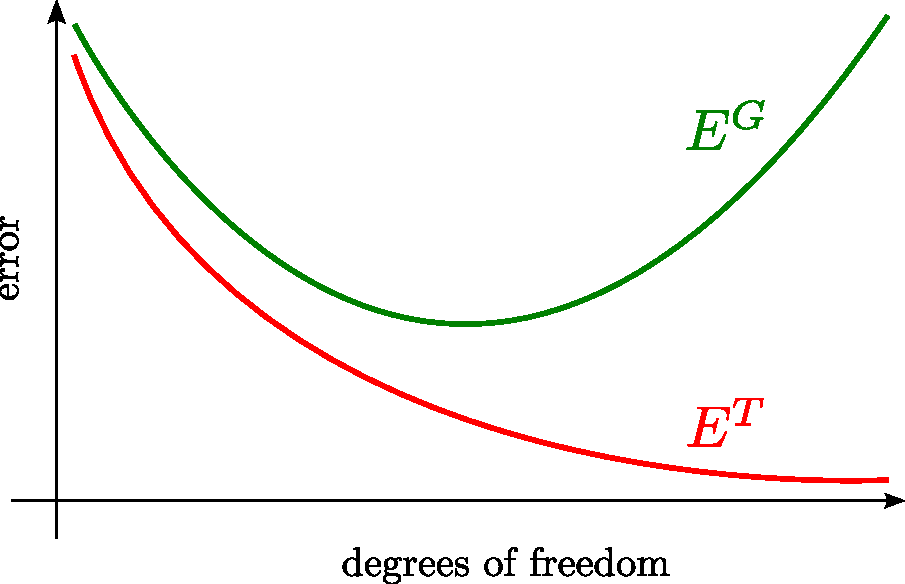
\includegraphics[width=0.5\textwidth]{img/bias_var_dog}
     \mode<article>{
	\caption{The bias-variance tradeoff with variable degrees of freedom}
	}
	\label{fig:bias_var_dog} 
\end{figure}

\end{frame}
\begin{frame}{\subsubsecname}

\begin{figure}[ht]
     \centering
	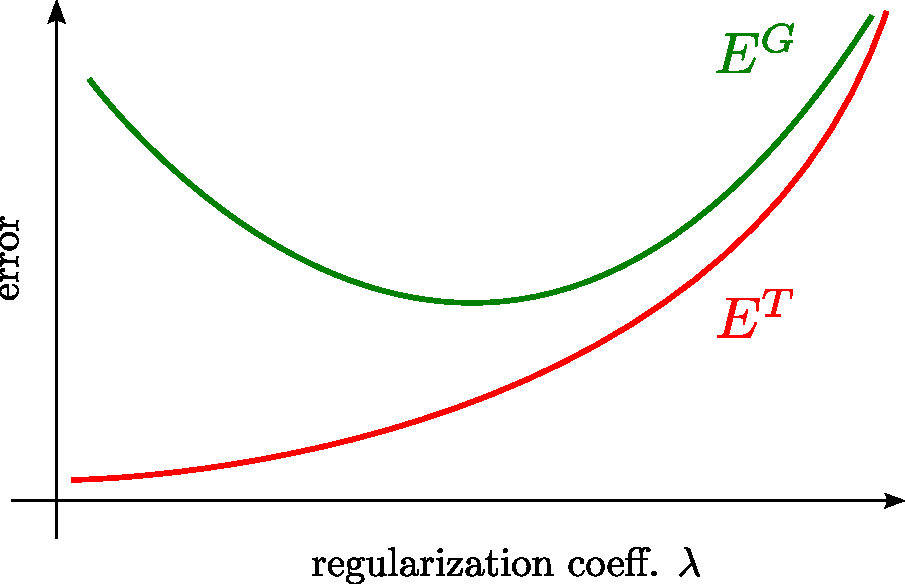
\includegraphics[width=0.5\textwidth]{img/bias_var_lambda}
     \mode<article>{
	\caption{The bias-variance tradeoff for different regularization strengths}
	}
	\label{fig:bias_var_lambda} 
\end{figure}

\end{frame}


\begin{frame}{\subsubsecname}

\begin{figure}[ht]
     \centering
	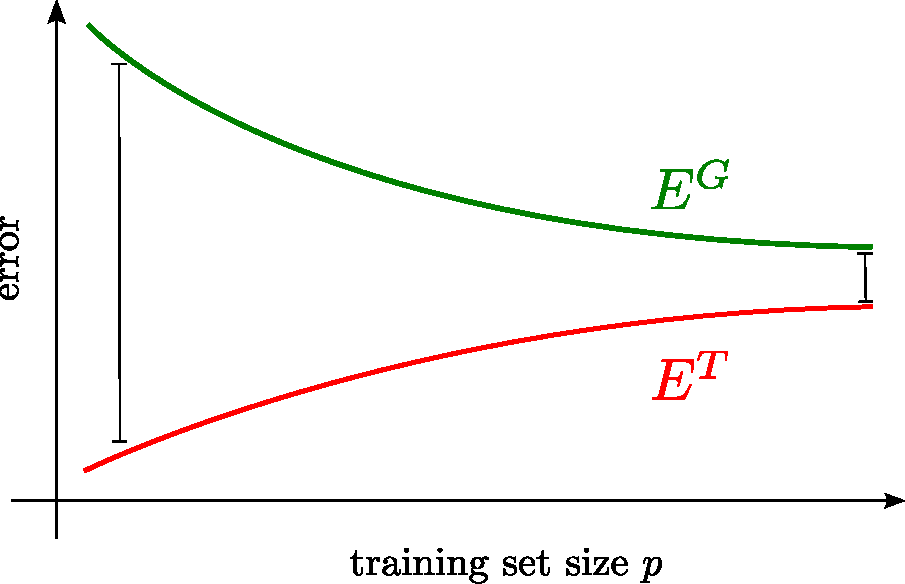
\includegraphics[width=0.5\textwidth]{img/bias_var_p_annot}
     \mode<article>{
	\caption{The bias-variance tradeoff for different number of training samples}
	}
	\label{fig:bias_var_p}
\end{figure}

\pause

\question{What is the benefit of looking at the bias-variance tradeoff as a function of $p$?}

\notesonly{
- Other than disentangling high bias from high variance, we also get an assessment of how much 
we would gain in generalization performance if we paid to increase the training set by x\% (i.e. cost-benefit analysis).
}

\end{frame}

\newpage

\subsection{Improving how we estimate $\widehat E^G$}

\begin{frame}

\question{Why should we care about how we estimate $\widehat E^G$?}

\notesonly{
- It's simply to identify potential overfitting or underfitting. Are we memorizing the training data or did we underestimate the complexity of function we're trying to fit? Once we identify what kind of problem we have with our model it implies which ``fixes'' are relevant and which would simply not help at all.
}

\end{frame}

% -----------------------------------------------------------------------------

\subsubsection{Testset method}

\begin{frame}\frametitle{Validation: Testset method}
	
	\begin{block}{Testset method (with hyperparameters, e.g. regularization coeff. $\lambda$)}
	
	3-way split of the data.
	
		\begin{enumerate}
		  \item training set: perform model selection for different values of $\lambda$
		  \item test set: select value of $\lambda $, 
		  		which provides best prediction results on this set $\leadsto \lambda^{\mathrm{opt}}$
		  \item validation set: estimate generalization performance of selected $\lambda$\\
		  This is data that was not used for model selection or hyperparameter selection.
		\end{enumerate}
	\end{block}	
	
	\vspace{1cm} 
	
	$ $\hspace{1cm}
	
\includegraphics[width=8cm]{img/traintestvalidation.pdf} \\
	
	Potential overfitting of $\lambda^{\mathrm{opt}}$ to test set.
\end{frame}

\subsubsection{$n$-fold cross-validation}

% -----------------------------------------------------------------------------
\begin{frame}
	\begin{block}{$n$-fold cross-validation for hyperparameter selection}
		\For{$\lambda = \lambda_1$ {\em\textbf{to}} $\lambda_n$}{
			perform $n$-fold cross-validation on 
				data with regularization $\lambda$
		}
		\vspace{2mm}

		pick optimal $\lambda^{\text{opt}}$ with minimum $\widehat{E}^G=\big<\widehat{E}^G_{k}\big>_{n folds}$\\
		\vspace{2mm}

		\textbf{final model:} train network on all data with $\lambda^{\text{opt}}$ 
	\end{block}
	
	\vspace{2mm}
	\begin{center}
		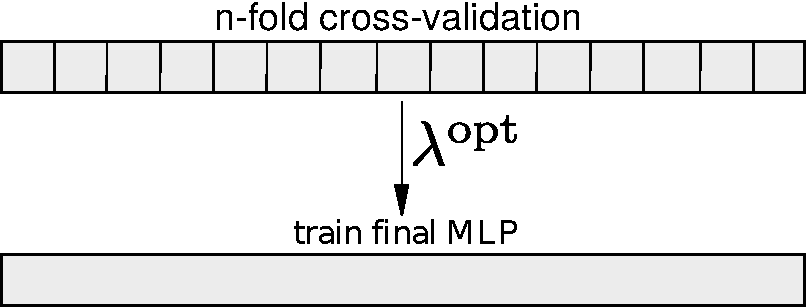
\includegraphics[width=8cm]{img/nfoldcrossvalidation.pdf} 
	\end{center}
	Optional: Additional validation set for estimating $\widehat{E}^G$ of final model.
\end{frame}

\newpage
% -----------------------------------------------------------------------------
\begin{frame}\frametitle{Validation: nested cross-validation}
	\begin{itemize}
	\item[\textcircled{1}]
	$ \begin{array}{ll}
		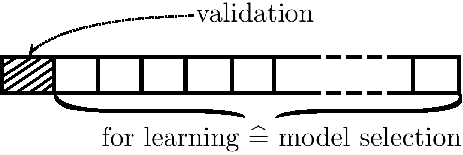
\includegraphics[height=1.2cm]{img/section1_fig34}
		& \begin{array}{ll}
			\bullet & \text{\footnotesize do n - 1 
				cross-validation for all values of } \lambda \\
			\bullet & \text{\footnotesize train with best $\lambda$} \\
			\bullet & \text{\footnotesize validate with learned model}
		\end{array}
	\end{array} $
	%\pause
	\item[\textcircled{2}]
	$ \begin{array}{ll}
		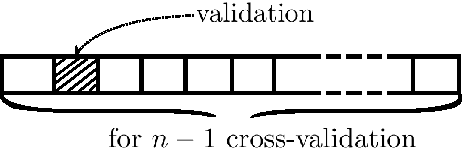
\includegraphics[height=1.2cm]{img/section1_fig35}
		& \begin{array}{ll}
			\bullet & \text{\footnotesize do n - 1 
				cross-validation for all values of } \lambda \\
			\bullet & \text{\footnotesize train with best $\lambda$} \\
			\bullet & \text{\footnotesize validate with learned model}
		\end{array}
	\end{array} $
	%\pause
	\item[\textcircled{n}]
	$ \begin{array}{ll}
		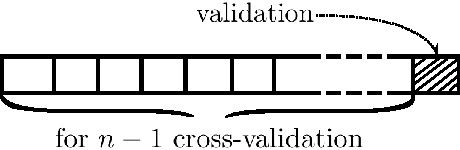
\includegraphics[height=1.2cm]{img/section1_fig36}
		& \begin{array}{ll}
			\bullet & \text{\footnotesize do n - 1
				cross-validation for all values of } \lambda \\
			\bullet & \text{\footnotesize train with best $\lambda$} \\
			\bullet & \text{\footnotesize validate with learned model}
		\end{array}
	\end{array} $
	\end{itemize}
	
	\begin{itemize}
		\item $\widehat{E}^G \quad\corresponds\quad$ 
			average over all $n$ validation errors
	\end{itemize}
\end{frame}

\mode<article>{
Every cross-validation (inner loop) above yields a model with some generalization performance.
The parameters (incl. hyperparameter selection) of each cross-validation can be different from the next.
The purpose of the outer loop is to estimate generalization performance that is less sensitive to the selection of the validation set, hyperparameter selection, and model selection procedure.
}

% -----------------------------------------------------------------------------
\begin{frame} 
	\begin{itemize}
		\item Never use test data for model selection 
			(including hyper-parameter search).
		\item Always embed the whole selection procedure (including 
			hyper-parameter search) within an $n$-fold cross-validation run.
		\item Watch out for validation data ``leaking'' into the training set.
		\mode<article>{
		Basing any decision (e.g. choice of hyperparameter values) based on the validation set is seen as validation data ``leaking'' into the training data. It has the potential of overfitting to the validation set which defeats the purpose of measuring performance on data that was never seen and did not influence any decisions. Performance that resembles that of the model when it is deployed and used with data outside of our control.
		}
	\end{itemize}
\end{frame}
